\graphicspath{{front_page}}

\thispagestyle{empty}

\widowpenalty=10000     % evita viudas (última línea sola al empezar la página siguiente)
\clubpenalty=10000
\brokenpenalty=10000

% Marca de agua
\newcommand\BackgroundPic{
    \put(0,0){
        \parbox[b][\paperheight]{\paperwidth}{
            \vfill
            \centering
            %\transparent{0.075} % Opacity level (0 = fully transparent, 1 = fully opaque)
            
\includegraphics[width=\paperwidth,keepaspectratio]{logos/upm_marca_de_agua.jpeg}
        }
    }
}

\AddToShipoutPicture*{\BackgroundPic} % Aplica fondo

% Logos arriba izquierda y derecha
\begin{minipage}{0.49\textwidth}
    
\includegraphics[width=3cm]{logos/logo_upm.png} % <- Logo izquierda
\end{minipage}
\hfill
\begin{minipage}{0.49\textwidth}
    \raggedleft
    
\includegraphics[width=3cm]{logos/logo_caminos.jpeg} % <- Logo derecha
\end{minipage}

\vspace{1cm}

% Título y subtítulo
\begin{center}
    {\LARGE\bfseries \longtitle}\\[1em]
    {\large \subtitle}
\end{center}

\vspace{0.5cm}

% Imagen centrada arriba
\begin{center}
    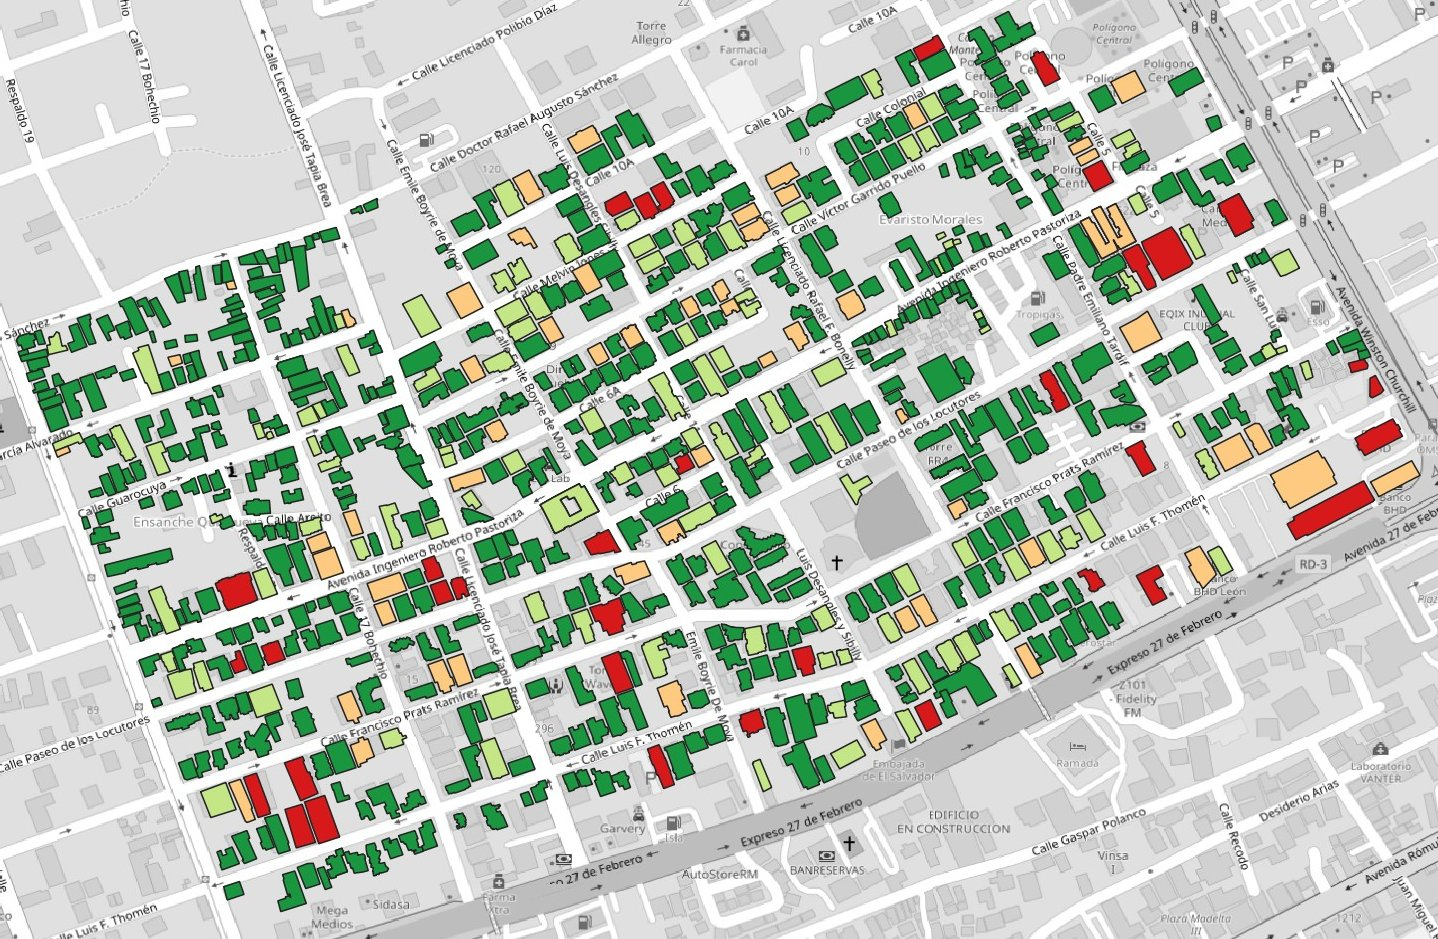
\includegraphics[width=0.8\textwidth]{front_page.jpg} % <- Imagen central
\end{center}

\vspace{0.5cm}



% Autor, tutor, asignatura, etc.
\begin{flushleft}
    \textbf{Author:} Miguel Ureña Pliego\\[0.5em]
    \textbf{Supervisor:} Miguel Marchamalo Sacristán\\[0.5em]
    \textbf{Academic year:} 2025-2026 \\[0.5em]
    \textbf{Degree:} MEng in Civil Engineering (Ingeniería de Caminos, Canales y Puertos)
\end{flushleft}

\vfill

% Universidad y facultad
\begin{center}
    \textbf{Universidad Politécnica de Madrid}\\
    ETSI de Caminos Canales y Puertos (Civil engineering school)
\end{center}
